Pour profiter des performances d'un \textsf{NoSQL}, il est essentiel
de définir à l'avance la nature et la représentation faite des données.
L'utilité et le choix du \textsf{NoSQL} doit principalement
réposer de la représentation des données. Adopter le \textsf{NoSQL} à
cause de la volumétrie ne garantit pas la performance et surtout la 
base perd l'intégrité qu'offre le modèle rélationnel.  
\\ 
\\ 
Les « \textsf{NoSQL} » offrent une autre façon
de représenter les données pour faciliter les accès et mises à jour des
données afin de gagner en performance. Le \textsf{NoSQL} n'est pas 
là pour remplacer systématiquement le  \textsf{SQL}. Pour la gestion des données 
organisée en tables, la structure des \textsf{SGBDR} y est exclusivement
dédiée. Cependant certaines solutions \textsf{NoSQL}, à l'image de \textsf{MongoDB}, ont
exhibé une charte de correspondance entre leurs composants et les composants \textsf{BDDR} 
\footnote{Database, Table, Index, colonne, clé
  primaire ...}. \textsf{MongoDB} a également mis
en place une charte de traduction requête \textsf{SQL} / requête
\textsf{MongoDB}.
\\
\\
\textsf{SQL} d'une part, \textsf{NoSQL} d'autre part, l'un n'exclut pas l'autre.
Tout dépend de l'usage qu'on compte en faire ou du profit qu'on
souhaite en tirer. Pour profiter à la fois du \textsf{NoSQL} et du \textsf{SQL}, il est très commun
de les faire cohabiter et de stocker
les données dans l'un ou dans l'autre en fonction des caractéristiques de 
celles-ci. C'est ce que fait d'ailleurs \textsf{Google} qui
même après avoir mis en place sa solution
propriétaire \textsf{BigTable} utilise \textsf{MySQL}
notamment pour son programme publicitaire \textsf{AdWords}, sa
principale source de revenue et qui utilise d'énormes quantités de
données. Cependant imaginer un protocole d'échange entre \textsf{SQL}
et \textsf{NoSQL} peut s'avérer très fastidieux dans la mesure où les
deux conçoivent les données très différemment.
\\
\\
Il existe une solution \textsf{Open Source} permettant des échanges
\textsf{SQL}/\textsf{NoSqL}: \textsf{Sqoop} ou « SQL To Hadoop
». \textsf{Hadoop}\index{Sqoop} est un assemblage de plusieurs
sous-projet avec à la base un système de
fichier \textsf{HDFS}\footnote{Hadoop Distributed File System}
et \textsf{HBASE} pour le stockage. Développé en \textsf{java}, sous
la direction de la fondation \textsf{Apache} et destiné aux
applications distribuées, sa structure de stockage \textsf{HBASE} est
un x\textsf{NoSQL} orienté colonnes. \textsf{Sqoop} charge
une table ou toute la base en système de fichiers \textsf{HDFS} en
fonction des options d'importation spécifiées et génère aussi des
classes \textsf{java} correspondantes aux tables de la bases, ainsi
que des objets correspondants aux lignes pour permettre d'interagir
avec les données importées.
\begin {figure}[H]
       \centering
        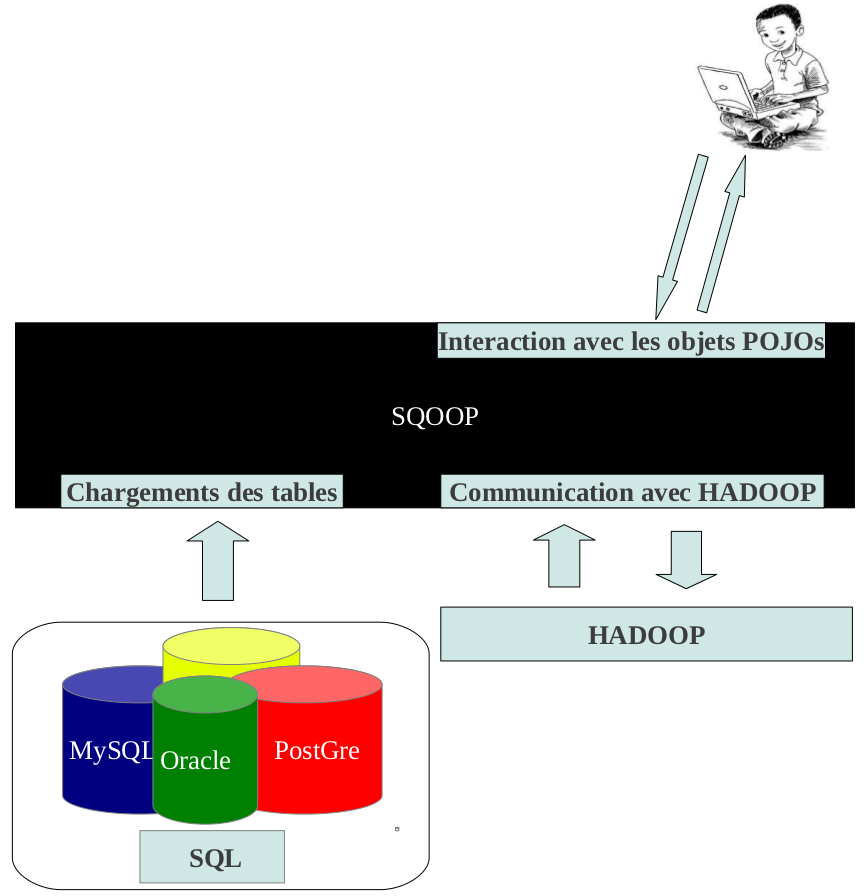
\includegraphics[scale=0.2]{\DIR/img/sqoop.png}	
        \caption{Fonctionnement de \textsf{SQOOP}}
	\label{sqoop}
  \end {figure}    
\noindent
Mise à part \textsf{Sqoop} qui est une solution pour \textsf{Hadoop}
d'échange avec le \textsf{SQL}, le framework
\textsf{spring} intègre des modules \textsf{Data access}\cite{springsource} permettant 
de faire persister des objets \textsf{POJO} dans des \textsf{BDD NoSQL}. En
exemple, le module \textsf{Spring Data MongoDB} permet de faire persister
les données dans \textsf{MongoDB}. Avec \textsf{spring} il est alors possible
d'effectuer une échange en deux temps:
\begin{enumerate}
\item D'abord transformer les données dans la \textsf{BDDR} en des objets 
      \textsf{POJO} par le biais de module déjà existant
      comme \textsf{hibernate, toplink, iBatis}...
\item Puis faire persister les objets \textsf{POJO} dans la base \textsf{NoSQL} par le biais du module 
      \textsf{Data access} dédié.    
\end{enumerate} 
Cependant il faut changer de module \textsf{Data access} à chaque fois
qu'il faut changer de \textsf{BDD NoSQL}. Il est difficile de mettre
en place une standardisation des interfaces dans la mesure où
chaque \textsf{BDD NoSQL} vient avec son propre langage de requête.
\begin {figure}[H]
       \centering
        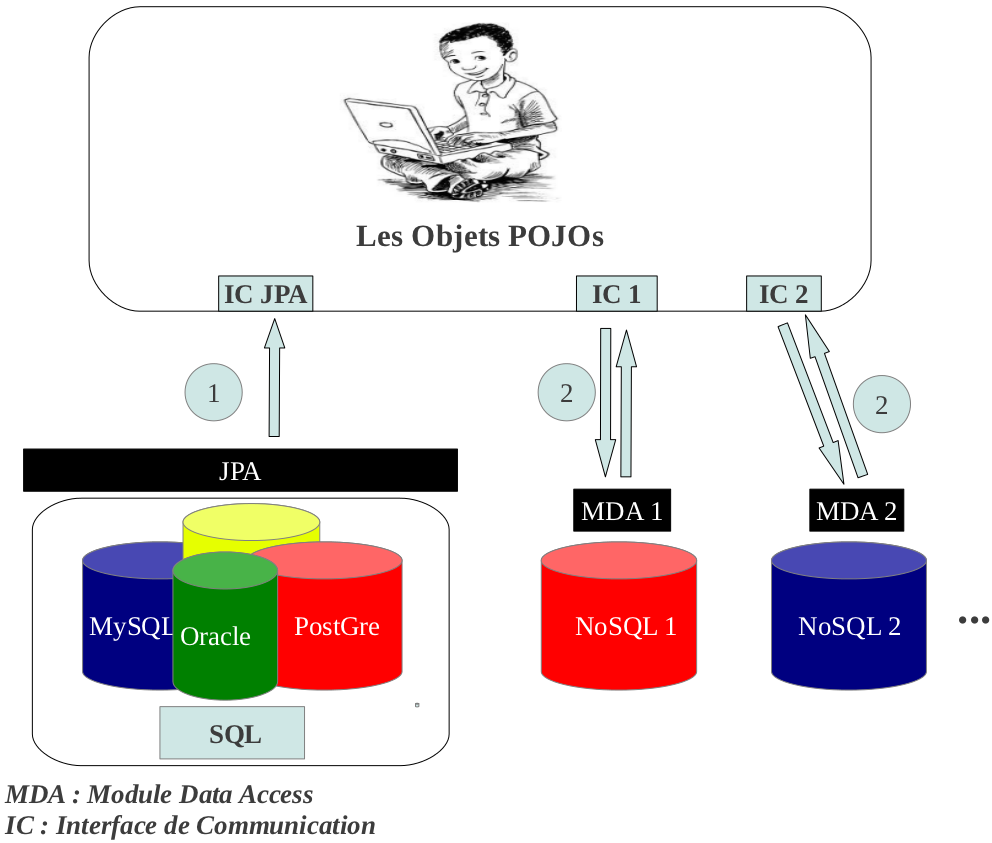
\includegraphics[scale=0.2]{\DIR/img/spring.png}	
        \caption{Possibilité d'échange \textsf{SQL/NoSQL} avec \textsf{spring}}
	\label{spring}
\end {figure}
